\section{Log Extension} \label{sec:log}
Now we shift our focus towards detecting some types of log misbehavior, namely,
omission attacks.\footnote{%
	TODO: we might need to clarify that, at some level, we are also dealing with
	omission attacks in the base design.  But what we are trying to detect is
	different here and in the base design.
} The design idea is an
extension of our base design.  A prerequisite is that the CT log landscape
is modified to support \emph{SCT cross-logging}.  Cross-logging refers to the
idea of logging signed statements in other logs to intertwine
them, thus making it more difficult to get away with
misbehavior.  We use the general idea and apply it to SCTs.  This means that
CTRs can log SFOs rather than certificate chains, making it possible to detect
MMD violations.

\subsection{Design Sketch}
Figure~\ref{fig:ext-log} provides an overview of the extended design.  Tor
Browser submits presented SFOs probabilistically to CTRs that are selected
at random, and CTRs mix the submitted SFOs before any auditing takes place.
Here, auditing refers to the submission of full SFOs rather than the underlying
certificate chains.  While phase~1 remains unchanged, there are minor changes
to the Tor consensus, phase~2, and phase~3.  The Tor consensus must include MMDs
of Tor Browser recognized logs, and CTRs should publish two additional metrics
in the extra-info document which are related to flooding.

\begin{figure*}
    \centering
    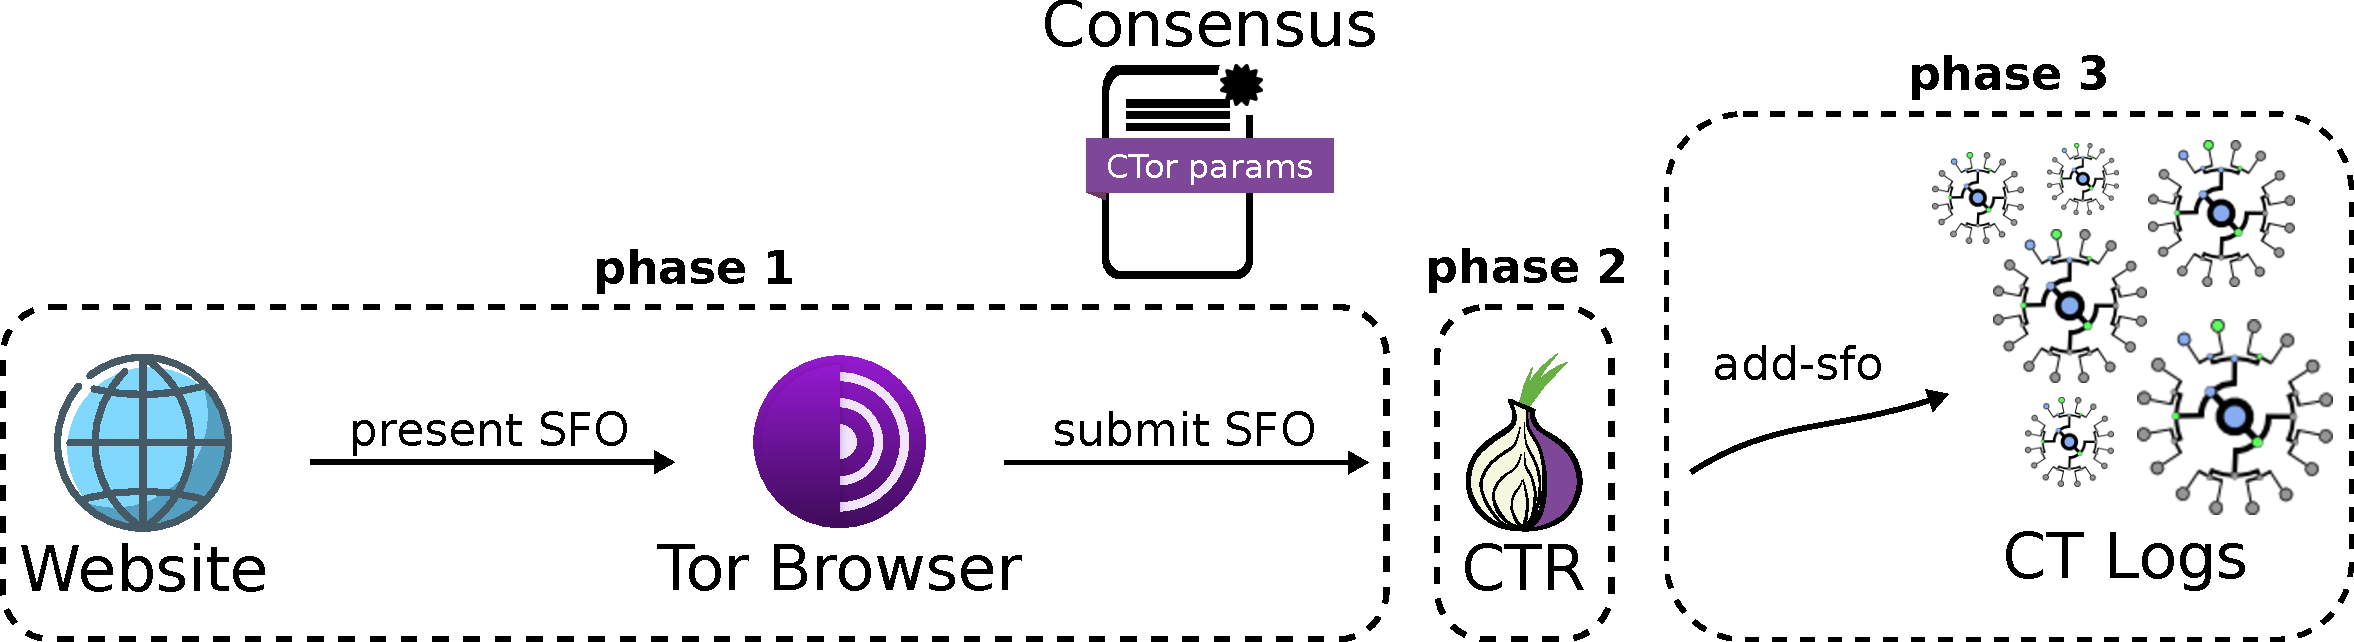
\includegraphics[width=0.85\textwidth]{img/design-log}
	\caption{TODO: Tobias, s/submit-entry/submit-sfo}
    \label{fig:ext-log}
\end{figure*}

Starting backwards with phase~3, CT logs need an endpoint that accepts SCTs in
addition to certificate chains.  We refer to this endpoint as
\texttt{submit-sfo}, and CTRs use it instead of \texttt{add-chain} or
\texttt{submit-entry}.  The submitted SCTs are of particular interest,
considering that they contain timestamps that reveal whether the issuing CT logs
violated their MMD promises by not incorporating a certificate chain on time.
Notably anyone can inspect the cross-logged SFOs, including existing CT
monitors, which in themselves prove whether a log misbehaved beyond doubt:
	an SCT is digitally signed by the issuing CT log, and
	it is cryptographically binding with regards to a certificate chain that
		is also public.

To increase the probability of catastrophic impact for the attacker by detecting
omissions, it is paramount that there are no \emph{early signals} that
allow the CT logs in question to reactively merge certificate chains before
any MMD is violated.  Therefore, \texttt{audit\_after} timestamps should be
computed as in Figure~\ref{fig:audit-after} with regards to the SCT and MMD that
yields the largest value (phase~2).

\begin{figure}
	\centering
	TODO: make pseudocode pretty
	\pseudocode[linenumbering, syntaxhighlight=auto]{%
		\pcif \textrm{SCT.timestamp} + \textrm{MMD} <
				\mathsf{now}():\\
			\pcind\textrm{t} \gets \mathsf{now}() +
				\mathsf{random\_delay}(\texttt{ct-delay-dist}) \\
		\pcelse\\
			\pcind \textrm{t} \gets \mathsf{now}() +
				\mathsf{MMD} +
				\mathsf{random\_delay}(\texttt{ct-delay-dist})
	}
	\caption{%
		Algorithm that computes an \texttt{audit\_after} timestamp $t$.
	}
	\label{fig:audit-after}
\end{figure}

As discussed next, the possibility of larger \texttt{audit\_after} timestamps
introduces the threat of network-wide flushes.  To facilitate detection, CTRs
should publish received and deleted SFO-bytes in the extra-info document.  This
can be compared to existing extra-info metrics, such as a Tor relay's
\texttt{read-history}.

\subsection{Security Analysis}
% MISC notes
% - Network-wide flush, detectable but hard to attribute
% - Requires that the logs extend their APIs to accept SCT cross-logging
